
\documentclass{article}
\usepackage[utf8]{inputenc}
\usepackage{minted}
\usepackage{graphicx}
\usepackage{hyperref}
\usepackage[dvipsnames]{xcolor}

\title{riot idosens}
\author{cmonaton }
\date{October 2019}

\begin{document}

\maketitle

\section{Introduction}
Installer l'os riot sur le détecteur d'ouverture de porte idosens. Cela permet entre autres d'utiliser la fonction radio du produit.

\section{Matériel}

\begin{figure}[H]
\begin{center}
\advance\leftskip-3cm
\advance\rightskip-3cm
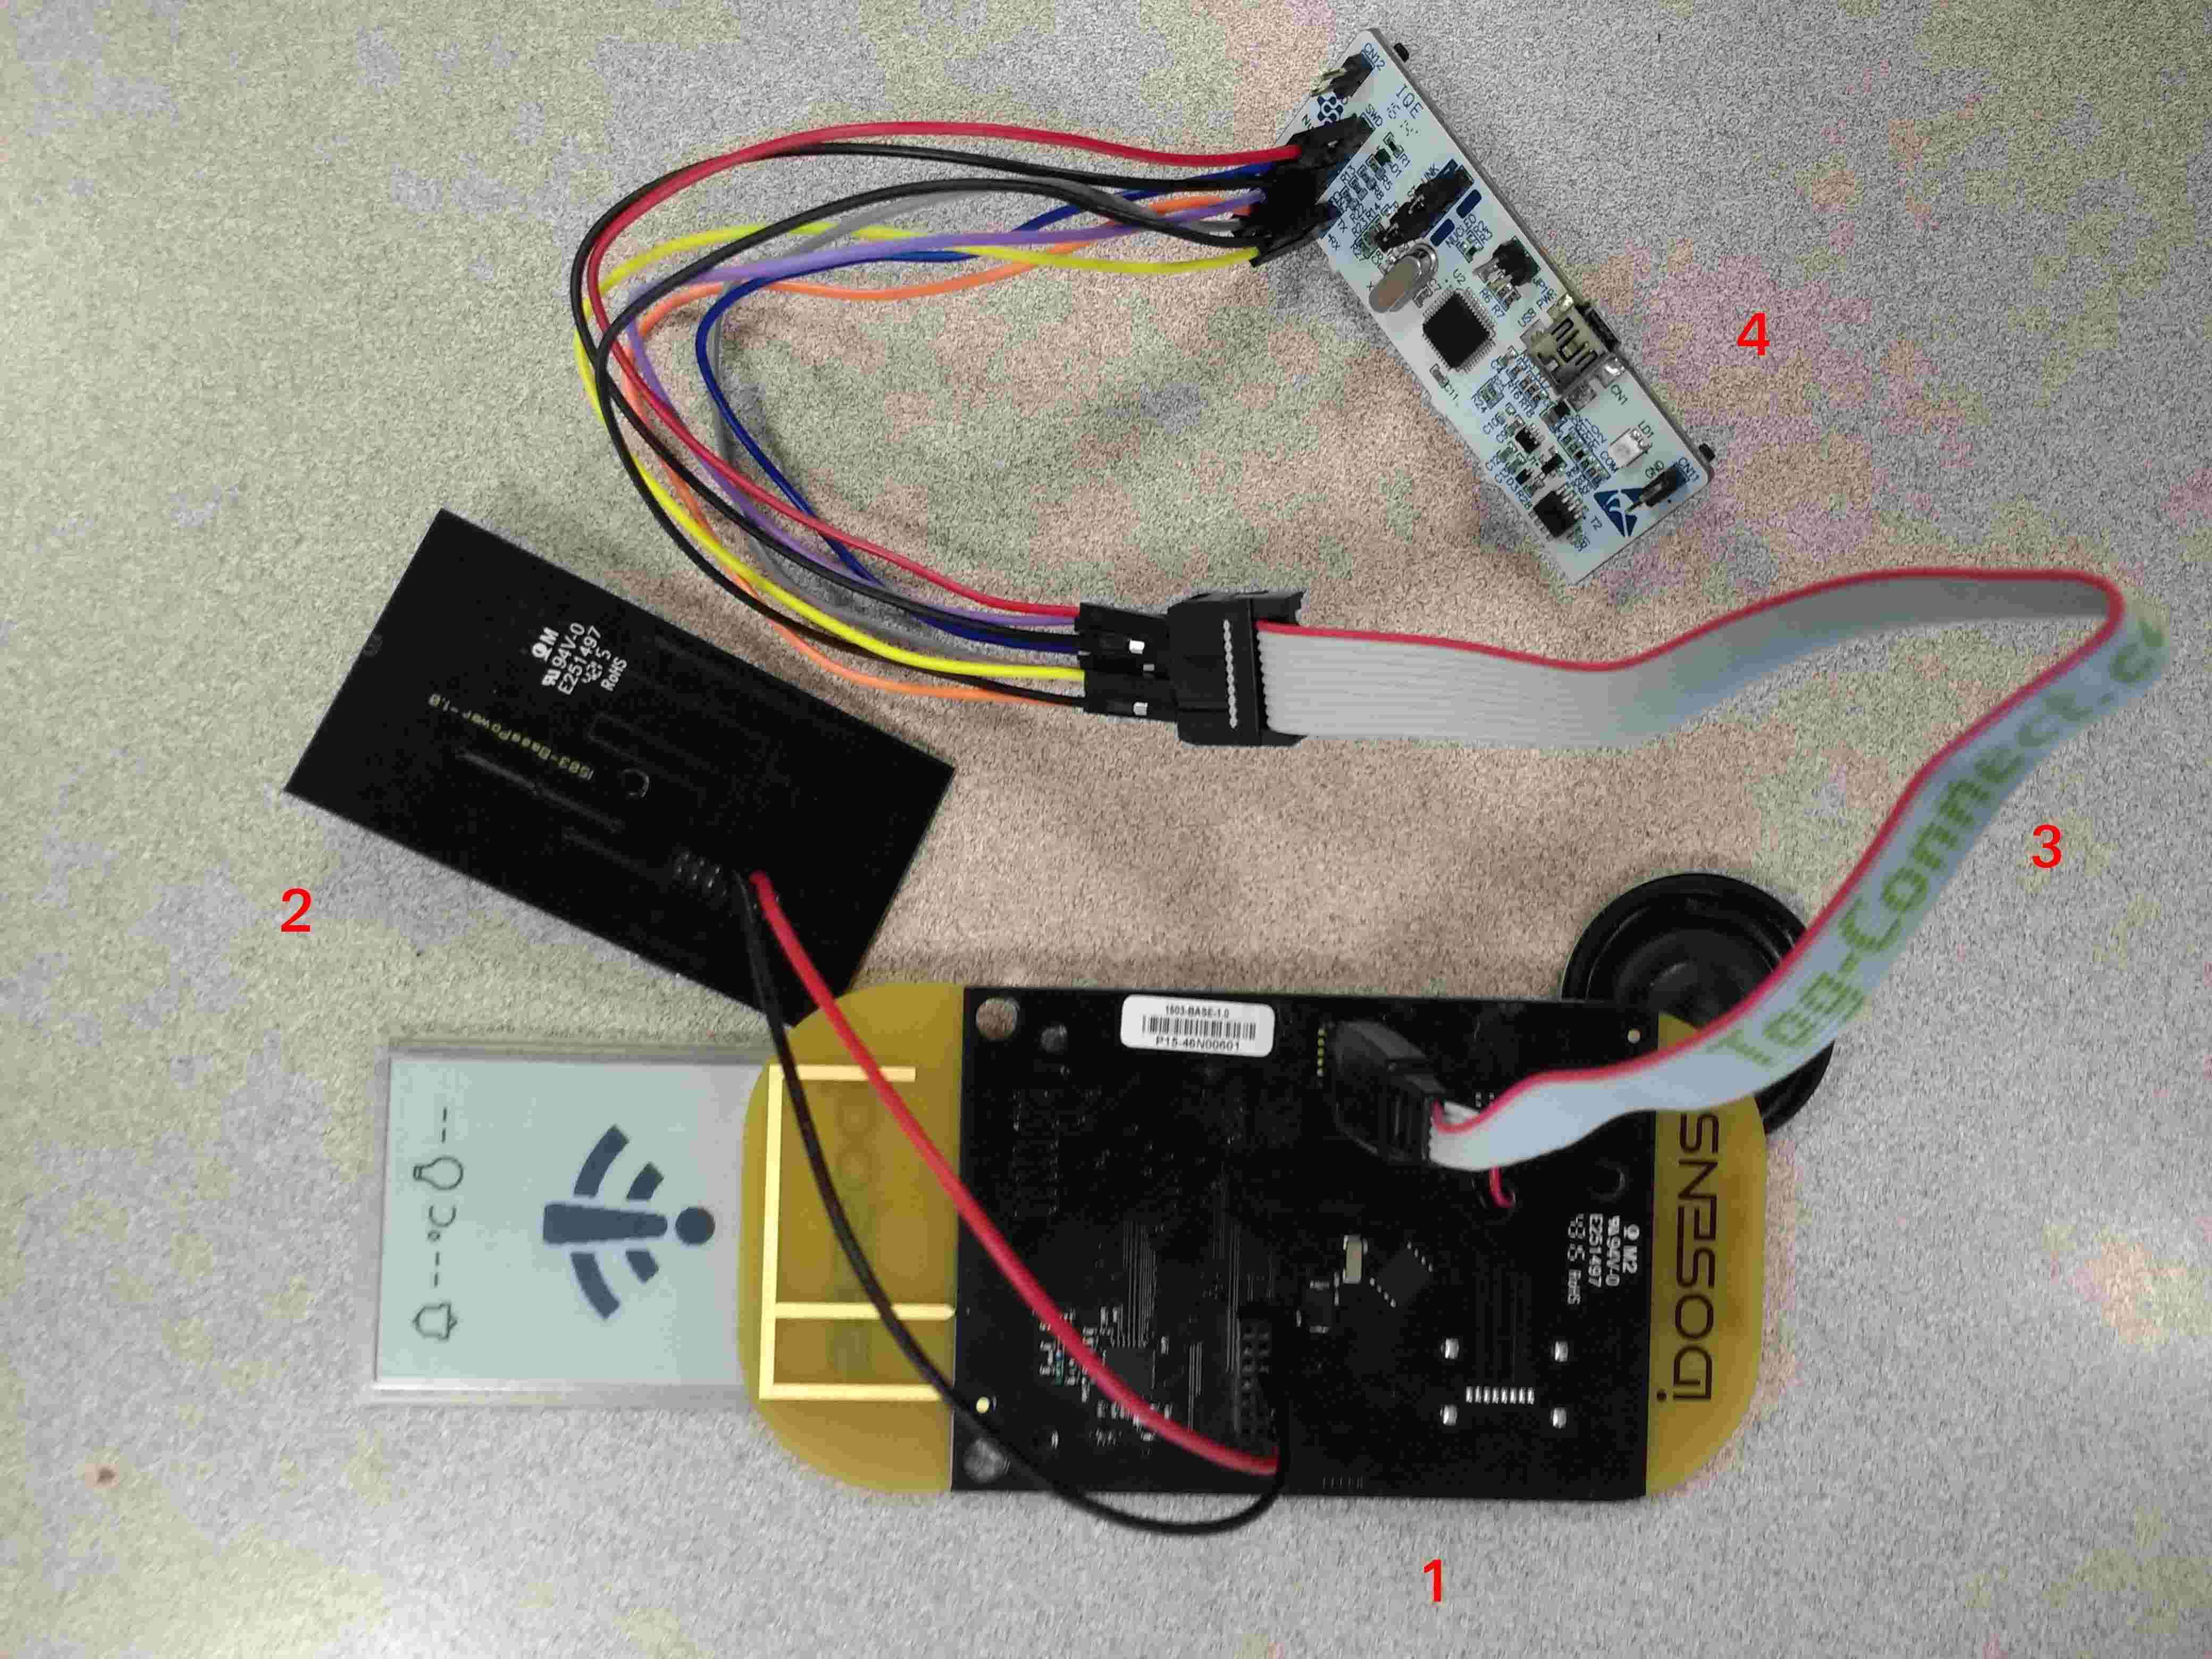
\includegraphics[keepaspectratio=true,scale=0.1]{idosens_numerote.jpg}
\label{visina8}
\end{center}\end{figure}

\begin{itemize}
    \item 1  Base
    \item{2} base power
    \item 3 Tag-connect
    \item 4 ST-LINK
\end{itemize}

\subsection{ST-LINK}
Ce débugueur/flasheur ST-LINK a été prélevé d'une carte nucleo :

\begin{figure}[H]
\begin{center}
\advance\leftskip-3cm
\advance\rightskip-3cm
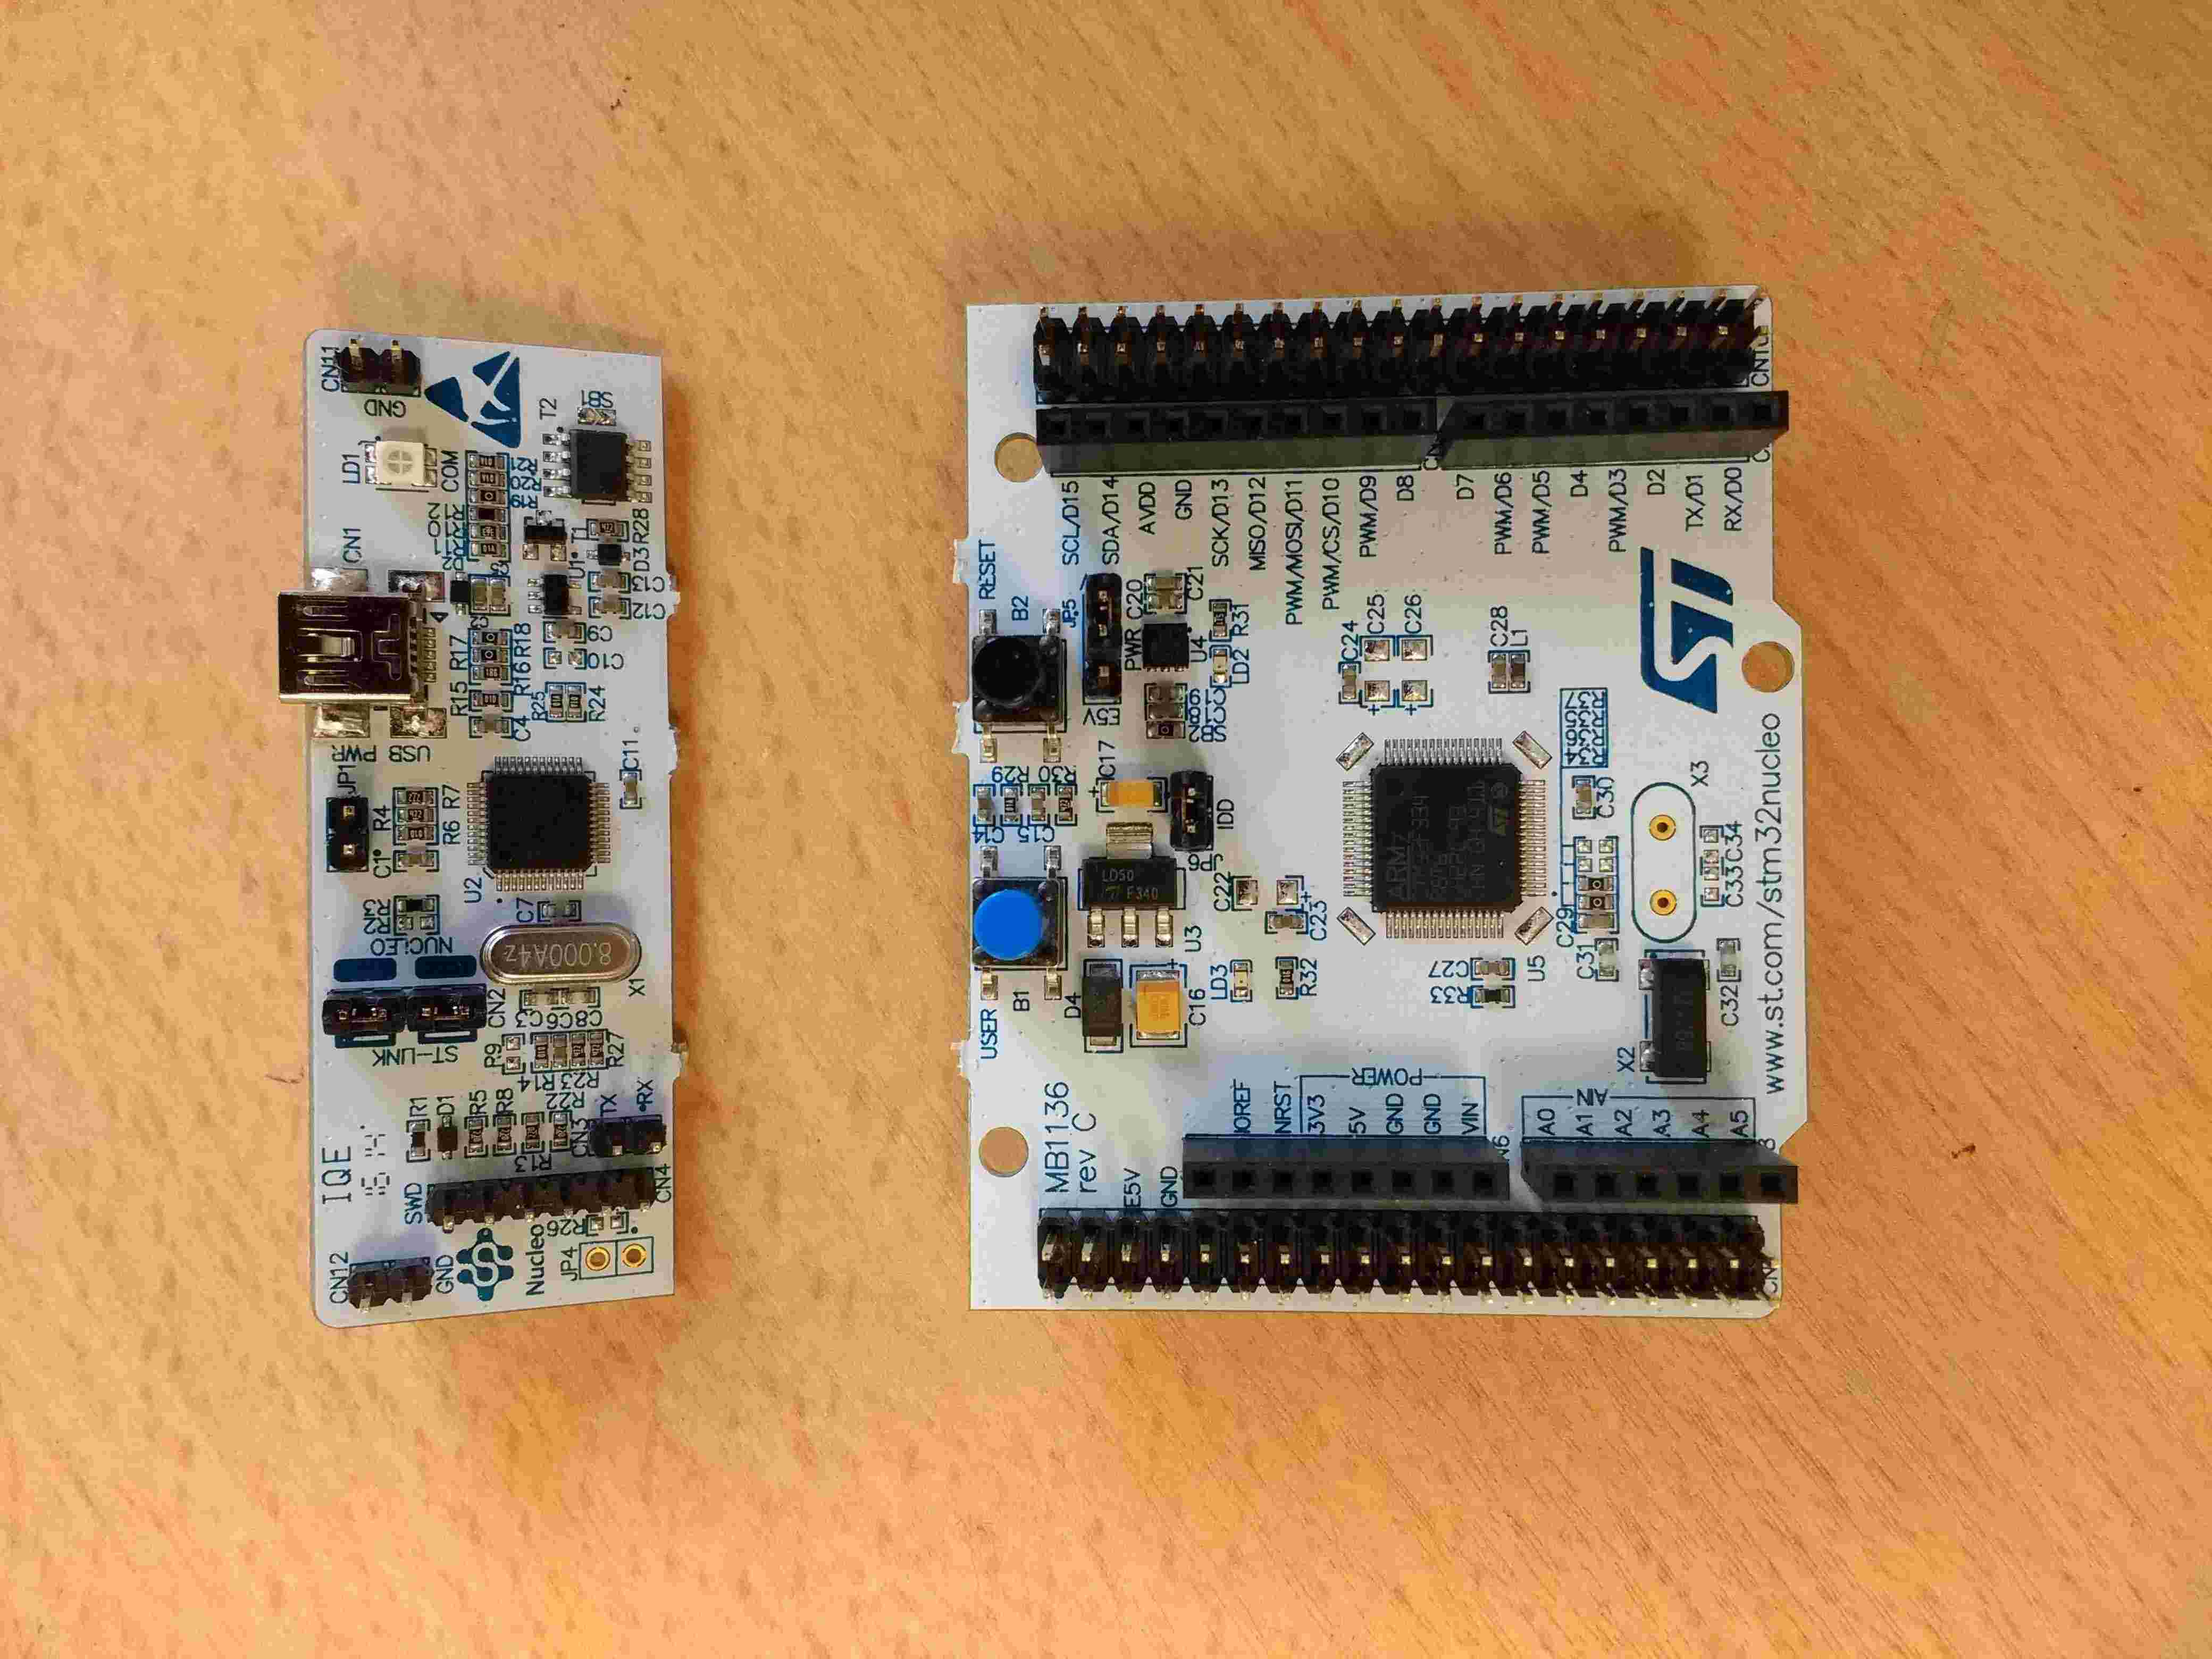
\includegraphics[keepaspectratio=true,scale=0.1]{nucleo_debug.jpg}
\label{visina8}
\end{center}\end{figure}

\subsection{Connexion base power}

\begin{figure}[H]
\begin{center}
\advance\leftskip-3cm
\advance\rightskip-3cm
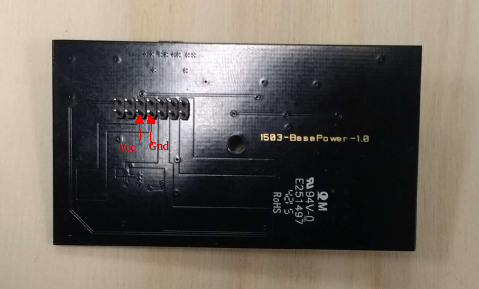
\includegraphics[keepaspectratio=true,scale=0.5]{power_dos_fleches.png}
\label{visina8}
\end{center}\end{figure}


\subsection {Connexion ST-LINK-Tag-connect}

Connectez le Tag-connect au nucleo selon ce tableau et selon les schémas des connecteurs :

\begin{figure}[H]
\begin{center}
\advance\leftskip-3cm
\advance\rightskip-3cm
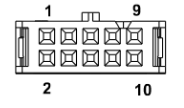
\includegraphics[keepaspectratio=true,scale=0.5]{tag_connectpinout.png}
\label{visina8}
\end{center}\end{figure}

\begin{figure}[H]
\begin{center}
\advance\leftskip-3cm
\advance\rightskip-3cm
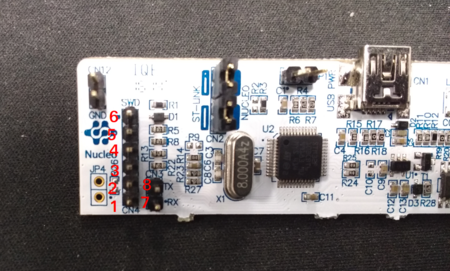
\includegraphics[keepaspectratio=true,scale=0.5]{Nucleo_pins.png}
\label{visina8}
\end{center}\end{figure}

\begin{center}
 \begin{tabular}{||c | c | c ||} 
 \hline
 Pin Nucleo  & Pin Tag-Connect \\ [0.8ex] 
 \hline\hline
  6 VDD TARGET   &  1 Vcc \\ 
 \hline
   3 SWDIO & 2 SWDIO \\
 \hline
  4 GND  & 3 Gnd\\
 \hline
  5 SWCLK  &  4 SWCLK\\
 \hline
  X  & X \\ [1ex] 
 \hline
  1 SWO  & 6 SWO \\ [1ex]
 \hline
  7 Rx  & 7 Tx \\ [1ex] 
 \hline
  X  & X \\ [1ex] 
 \hline
 8 Tx & 9 Rx \\ [1ex] 
 \hline
 2 NRST & 10 NRST\\ [1ex] 
 \hline
\end{tabular}
\end{center}



\section{installation logiciels et configuration du PC}
J'utilise ubuntu 16.04
\subsection{Déverouiller ports USB}




ajoutez un fichier 50-myusb.rules dans 

\begin{minted}{bash}
/etc/udev/rules.d

\end{minted}
contenant 

\begin{minted}{bash}
ACTION=="add", KERNEL=="ttyACM[0-9]*", ATTRS{idVendor}=="0483",
ATTRS{idProduct}=="374b", MODE="0666"

\end{minted}

avec idProduct et idVendor à renseigner en fonction du votre produit. On les trouve avec le programme

\begin{minted}{bash}
lsusb

\end{minted}
Redémarrez le PC.
\subsection{Installer le compilateur arm-none-eabi-gcc pour générer du code pour la carte}

\begin{minted}{bash}
sudo apt-get install gcc-arm-none-eabi

\end{minted}


\subsection{Installer pyserial pour communiquer avec la carte}

\begin{minted}{bash}
sudo apt-get install python3-pip
python3 -m pip install pyserial
\end{minted}

\section{Compiler et utiliser riot}


Téléchargez le code à : \url{https://github.com/GitClementtest/riot_idosens}\\
Dans un terminal, allez dans 

\begin{minted}{bash}
 extractionPath/riot_idosens/tests/driver_sx127x/
\end{minted}



Pour lancer la compilation et flasher la carte :
\begin{minted}{bash}
make BOARD=idosens flash term
\end{minted}



\end{document}
